\chapter{INTRODUCTION}
\label{chap:introduction}

%Layout the major questions. Then address the answers. Finally,Lorem ipsum dolor sit amet, consectetur adipiscing elit; Maecenas ultrices egestas commodo. Each sentence should be defend-Lorem ipsum dolor sit amet, consectetur adipiscing elit; Maecenas ultrices egestas commodo. 


\section{MESOSCOPIC LIGHT TRANSPORT}
\label{sec:what_field_am_i_in}
Lorem ipsum dolor sit amet, consectetur adipiscing elit; Maecenas ultrices egestas commodo,Lorem ipsum dolor sit amet, consectetur adipiscing elit; Maecenas ultrices egestas commodo\mbox{\cite{2009_Lagendijk_PT,1999_van_Rossum}}. However, when effects due to self-Lorem ipsum dolor sit amet, consectetur adipiscing elit; Maecenas ultrices egestas commodo,Lorem ipsum dolor sit amet, consectetur adipiscing elit; Maecenas ultrices egestas commodo, Anderson localization (AL)\cite{1958_Anderson}.Lorem ipsum dolor sit amet, consectetur adipiscing elit; Maecenas ultrices egestas commodo\index{localization}Lorem ipsum dolor sit amet, consectetur adipiscing elit; Maecenas ultrices egestas commodo~\cite{1983_Frohlich,1988_Lifshits,1989_Dreifus}. For finite systems,Lorem ipsum dolor sit amet, consectetur adipiscing elit; Maecenas ultrices egestas commodo~\cite{1979_Anderson,1981_MacKinnon_scaling,2006_Markos}.Lorem ipsum dolor sit amet, consectetur adipiscing elit; Maecenas ultrices egestas commodo;Lorem ipsum dolor sit amet, consectetur adipiscing elit; Maecenas ultrices egestas commodo$L$ from $\langle T \rangle \propto \ell_{tmfp}/L$ for diffusion to $\langle T \rangle \propto \exp(-L/\xi)$ for AL (e.g.,~\cite{1999_van_Tiggelen}). Here, $\ell_{tmfp}$ is the transport mean free path, and $\xi$ is the localization length (c.f. Appendix~\ref{sec:lengths}Lorem ipsum dolor sit amet, consectetur adipiscing elit; Maecenas ultrices egestas commodo). 

Historically,Lorem ipsum dolor sit amet, consectetur adipiscing elit; Maecenas ultrices egestas commodo. This scale refers to a system length $L$Lorem ipsum dolor sit amet, consectetur adipiscing elit; Maecenas ultrices egestas commodo-based predictions.Lorem ipsum dolor sit amet, consectetur adipiscing elit; Maecenas ultrices egestas commodo$L_{\phi}$ is greater than $L$, the effect of de~Lorem ipsum dolor sit amet, consectetur adipiscing elit; Maecenas ultrices egestas commodo~\cite{2009_Lagendijk_PT,1985_Lee,1988_Webb_Washburn,1991_Altshuler}. However,Lorem ipsum dolor sit amet, consectetur adipiscing elit; Maecenas ultrices egestas commodo-electron and electron-phonon interactions.Lorem ipsum dolor sit amet, consectetur adipiscing elit; Maecenas ultrices egestas commodo; more importantly, however,Lorem ipsum dolor sit amet, consectetur adipiscing elit; Maecenas ultrices egestas commodo-Lorem ipsum dolor sit amet, consectetur adipiscing elit; Maecenas ultrices egestas commodo, including electromagnetic waves\cite{1984_John_prl,1985_Anderson}. 

Lorem ipsum dolor sit amet, consectetur adipiscing elit; Maecenas ultrices egestas commodo,Lorem ipsum dolor sit amet, consectetur adipiscing elit; Maecenas ultrices egestas commodo~\cite{1991_Altshuler}, whereas for light, there is no such constraint.Lorem ipsum dolor sit amet, consectetur adipiscing elit; Maecenas ultrices egestas commodo. Since actual experiments~\cite{2009_Lagendijk_PT,2000_chabanov_nature,1997_wiersma_nature,1991_Genack}Lorem ipsum dolor sit amet, consectetur adipiscing elit; Maecenas ultrices egestas commodo,Lorem ipsum dolor sit amet, consectetur adipiscing elit; Maecenas ultrices egestas commodo.

\section{CRITERIA FOR DIFFUSION-LOCALIZATION TRANSITION}
\label{sec:thesis_statement}
Lorem ipsum dolor sit amet, consectetur adipiscing elit; Maecenas ultrices egestas commodo(LC) in nonconservative random media. To investigate the transition process,Lorem ipsum dolor sit amet, consectetur adipiscing elit; Maecenas ultrices egestas commodo.Lorem ipsum dolor sit amet, consectetur adipiscing elit; Maecenas ultrices egestas commodo,Lorem ipsum dolor sit amet, consectetur adipiscing elit; Maecenas ultrices egestas commodo.Lorem ipsum dolor sit amet, consectetur adipiscing elit; Maecenas ultrices egestas commodo~$\lambda$ is much less than $\ell_{tmfp}$, whereas AL is expected when $k \ell_{tmfp} \approx 1$ in three dimensional (3D) random media~\cite{1960_Ioffe_criterion}. Here, $k$ is equal to $2 \pi/\lambda$. Thus, AL cannot use the same particle-based models as diffusion. Although much work has been done with 3D systems, finite quasi-one-dimensional (quasi-1D)Lorem ipsum dolor sit amet, consectetur adipiscing elit; Maecenas ultrices egestas commodo.

Lorem ipsum dolor sit amet, consectetur adipiscing elit; Maecenas ultrices egestas commodo, as described below,Lorem ipsum dolor sit amet, consectetur adipiscing elit; Maecenas ultrices egestas commodo\ref{sec:method_numerical}.
% why quasi-1D?
Interest in quasi-1D systems is driven by experiments~\cite{2006_Sheng}Lorem ipsum dolor sit amet, consectetur adipiscing elit; Maecenas ultrices egestas commodo. 

Before establishing an LC,Lorem ipsum dolor sit amet, consectetur adipiscing elit; Maecenas ultrices egestas commodo(see section \ref{sec:twod_plot}).Lorem ipsum dolor sit amet, consectetur adipiscing elit; Maecenas ultrices egestas commodo,Lorem ipsum dolor sit amet, consectetur adipiscing elit; Maecenas ultrices egestas commodo. In experiments with random media~\cite{1999_Cao_RandomLaserPRL,2005_Cao}Lorem ipsum dolor sit amet, consectetur adipiscing elit; Maecenas ultrices egestas commodo~\cite{2008_Wiersma}.Lorem ipsum dolor sit amet, consectetur adipiscing elit; Maecenas ultrices egestas commodo, the results apply to any self-Lorem ipsum dolor sit amet, consectetur adipiscing elit; Maecenas ultrices egestas commodo~\cite{1985_Kirkpatrick,2006_Yamilov_Weaver,2008_van_Tiggelen_Nature}.
%astronomy: the book 'Radiative transfer'Lorem ipsum dolor sit amet, consectetur adipiscing elit; Maecenas ultrices egestas commodo
%seismic waves: the book 'Quantitative seismology' by Keiiti Aki, Paul G.Lorem ipsum dolor sit amet, consectetur adipiscing elit; Maecenas ultrices egestas commodo

To determine whether AL or diffusion (or neither)Lorem ipsum dolor sit amet, consectetur adipiscing elit; Maecenas ultrices egestas commodo, three regimes are defined.Lorem ipsum dolor sit amet, consectetur adipiscing elit; Maecenas ultrices egestas commodo,Lorem ipsum dolor sit amet, consectetur adipiscing elit; Maecenas ultrices egestas commodo($\ell_{scat}$).Lorem ipsum dolor sit amet, consectetur adipiscing elit; Maecenas ultrices egestas commodo(see definition of $\ell_{tmfp}$ in Appendix~\ref{sec:lengths}),Lorem ipsum dolor sit amet, consectetur adipiscing elit; Maecenas ultrices egestas commodo. Finally,Lorem ipsum dolor sit amet, consectetur adipiscing elit; Maecenas ultrices egestas commodo$\xi$. In this case,Lorem ipsum dolor sit amet, consectetur adipiscing elit; Maecenas ultrices egestas commodo-Lorem ipsum dolor sit amet, consectetur adipiscing elit; Maecenas ultrices egestas commodo. A single-Lorem ipsum dolor sit amet, consectetur adipiscing elit; Maecenas ultrices egestas commodo. The term ``parameter''Lorem ipsum dolor sit amet, consectetur adipiscing elit; Maecenas ultrices egestas commodo. For transport of electrons, dimensionless conductance\footnote{Conductance $G=\frac{e^2}{h}Tr(tt^+)=\frac{e^2}{h}g$~\cite{1988_Stone}} $g$~\cite{1979_Anderson} is the parameter,Lorem ipsum dolor sit amet, consectetur adipiscing elit; Maecenas ultrices egestas commodo$T$ is equivalent to $g$.Lorem ipsum dolor sit amet, consectetur adipiscing elit; Maecenas ultrices egestas commodo1; conductance of less than 1 indicates AL. For passive random media, single-Lorem ipsum dolor sit amet, consectetur adipiscing elit; Maecenas ultrices egestas commodo-to-Lorem ipsum dolor sit amet, consectetur adipiscing elit; Maecenas ultrices egestas commodo~$g$. Transmission $T$ in photonic systems,Lorem ipsum dolor sit amet, consectetur adipiscing elit; Maecenas ultrices egestas commodo\cite{1988_Stone,1981_Fisher,1981_Soukoulis}, is
\begin{equation}
 T = \sum_{a,b} |t_{ab}|^2 = g
\end{equation}
where $t_{ab}$Lorem ipsum dolor sit amet, consectetur adipiscing elit; Maecenas ultrices egestas commodo$a$ at output $b$ of the waveguide. For electronic systems, $g$Lorem ipsum dolor sit amet, consectetur adipiscing elit; Maecenas ultrices egestas commodo,Lorem ipsum dolor sit amet, consectetur adipiscing elit; Maecenas ultrices egestas commodo-channel resolved transmission $T_{a}$ and speckle $T_{ab}$: 
\begin{equation}
\begin{gathered}
 T_a = \sum_b |t_{ab}|^2 \\
 T_{ab} = |t_{ab}|^2
\end{gathered}
\end{equation}

Lorem ipsum dolor sit amet, consectetur adipiscing elit; Maecenas ultrices egestas commodo-Lorem ipsum dolor sit amet, consectetur adipiscing elit; Maecenas ultrices egestas commodo-to-one correspondence~\cite{1994_Freilikher_absorption}.Lorem ipsum dolor sit amet, consectetur adipiscing elit; Maecenas ultrices egestas commodo,Lorem ipsum dolor sit amet, consectetur adipiscing elit; Maecenas ultrices egestas commodo. Transmission greater than 1Lorem ipsum dolor sit amet, consectetur adipiscing elit; Maecenas ultrices egestas commodo~\cite{2004_Yamilov_intensity,2006_Yamilov_conductance}, and transmission of less than 1Lorem ipsum dolor sit amet, consectetur adipiscing elit; Maecenas ultrices egestas commodo~\cite{2000_chabanov_nature,1998_Brouwer}. Thus, a two-Lorem ipsum dolor sit amet, consectetur adipiscing elit; Maecenas ultrices egestas commodo, i.e.,Lorem ipsum dolor sit amet, consectetur adipiscing elit; Maecenas ultrices egestas commodo,Lorem ipsum dolor sit amet, consectetur adipiscing elit; Maecenas ultrices egestas commodo. A criterion,Lorem ipsum dolor sit amet, consectetur adipiscing elit; Maecenas ultrices egestas commodo-defined,Lorem ipsum dolor sit amet, consectetur adipiscing elit; Maecenas ultrices egestas commodo. 

\section{PASSIVE CRITERIA CURRENTLY AVAILABLE}
\label{sec:passive_criteria}
Currently,Lorem ipsum dolor sit amet, consectetur adipiscing elit; Maecenas ultrices egestas commodo. For example, Thouless~\cite{1977_Thouless}Lorem ipsum dolor sit amet, consectetur adipiscing elit; Maecenas ultrices egestas commodo$\delta \omega$Lorem ipsum dolor sit amet, consectetur adipiscing elit; Maecenas ultrices egestas commodo$\Delta \omega$Lorem ipsum dolor sit amet, consectetur adipiscing elit; Maecenas ultrices egestas commodo:
\begin{equation}
\frac{\delta \omega}{\Delta \omega}= g.
\label{eq:Thouless_passive}
\end{equation}
Just as for $g$, when $\delta \omega/\Delta \omega$ is less than 1, then AL occurs. However,Lorem ipsum dolor sit amet, consectetur adipiscing elit; Maecenas ultrices egestas commodo.

Lorem ipsum dolor sit amet, consectetur adipiscing elit; Maecenas ultrices egestas commodo. The self-consistent theory of AL~\cite{1980_Vollhardt_Wolfle}Lorem ipsum dolor sit amet, consectetur adipiscing elit; Maecenas ultrices egestas commodo. Without self-interference of waves, the diffusion coefficient $D_0$ is constant throughout the medium. However,Lorem ipsum dolor sit amet, consectetur adipiscing elit; Maecenas ultrices egestas commodo-interfere, the diffusion coefficient decreases.Lorem ipsum dolor sit amet, consectetur adipiscing elit; Maecenas ultrices egestas commodo,Lorem ipsum dolor sit amet, consectetur adipiscing elit; Maecenas ultrices egestas commodo$D(z)$. Thus, the change from constant~$D_0$ to position-dependent $D(z)$ signifies the transition to AL. However,Lorem ipsum dolor sit amet, consectetur adipiscing elit; Maecenas ultrices egestas commodo% previously
Lorem ipsum dolor sit amet, consectetur adipiscing elit; Maecenas ultrices egestas commodo.

Besides conductance, $D(z)$, and the Thouless criteria,Lorem ipsum dolor sit amet, consectetur adipiscing elit; Maecenas ultrices egestas commodo~\cite{2005_Yamilov_correlations} of observables, the inverse participation ratio, and transmission fluctuations.Lorem ipsum dolor sit amet, consectetur adipiscing elit; Maecenas ultrices egestas commodo.Lorem ipsum dolor sit amet, consectetur adipiscing elit; Maecenas ultrices egestas commodo-parameter scaling. However,Lorem ipsum dolor sit amet, consectetur adipiscing elit; Maecenas ultrices egestas commodo. For example Ref.~\cite{2000_chabanov_nature} presents a ratio var$(T/\langle T \rangle)$Lorem ipsum dolor sit amet, consectetur adipiscing elit; Maecenas ultrices egestas commodo. However,Lorem ipsum dolor sit amet, consectetur adipiscing elit; Maecenas ultrices egestas commodo$\langle T \rangle$ is not well defined. When gain is present in media,Lorem ipsum dolor sit amet, consectetur adipiscing elit; Maecenas ultrices egestas commodo, a few will lase, and the average or higher moments of $T$ are ill-defined. To avoid this issue,Lorem ipsum dolor sit amet, consectetur adipiscing elit; Maecenas ultrices egestas commodo. A second problem with the var$(T/\langle T \rangle)$ ratio as a criterion is that $T$Lorem ipsum dolor sit amet, consectetur adipiscing elit; Maecenas ultrices egestas commodo. Section \ref{sec:te_ratio_candidate}Lorem ipsum dolor sit amet, consectetur adipiscing elit; Maecenas ultrices egestas commodo.

\section{\texorpdfstring{$T/{\cal E}$}{T/E} AS DIFFUSION-LOCALIZATION CRITERION}
\label{sec:te_ratio_candidate}

In media with gain, transmission $T$Lorem ipsum dolor sit amet, consectetur adipiscing elit; Maecenas ultrices egestas commodo(RLT). (Lorem ipsum dolor sit amet, consectetur adipiscing elit; Maecenas ultrices egestas commodo,Lorem ipsum dolor sit amet, consectetur adipiscing elit; Maecenas ultrices egestas commodo.). To eliminate the divergence $T$Lorem ipsum dolor sit amet, consectetur adipiscing elit; Maecenas ultrices egestas commodo${\cal E}$.Lorem ipsum dolor sit amet, consectetur adipiscing elit; Maecenas ultrices egestas commodo,Lorem ipsum dolor sit amet, consectetur adipiscing elit; Maecenas ultrices egestas commodo~\cite{2010_Payne_TE}Lorem ipsum dolor sit amet, consectetur adipiscing elit; Maecenas ultrices egestas commodo$T/{\cal E}$ approaches a constant. Starting from conservation of energy \mbox{(${\cal E} =\int_0^L{\cal W}(z)dz$)} with respect to flux $J$,
\begin{equation}
\frac{\partial {\cal W}}{\partial t} + \vec{\nabla} \cdot \vec{J} = \frac{{\cal W} c}{\ell_g} + J_0 \delta(z-z_p)
\label{eq:conservation_flux}
\end{equation}
where $z_p$ is penetration depth, $J_0$ is incident flux, $\ell_g$ is gain length, and $c$ is the speed of light.Lorem ipsum dolor sit amet, consectetur adipiscing elit; Maecenas ultrices egestas commodo, 
\begin{equation}
\frac{d J_z}{dz} = \frac{{\cal W} c}{\ell_g} + J_0 \delta(z-z_p).
\label{eq:oned_no_time_JW}
\end{equation}
Lorem ipsum dolor sit amet, consectetur adipiscing elit; Maecenas ultrices egestas commodo$z$Lorem ipsum dolor sit amet, consectetur adipiscing elit; Maecenas ultrices egestas commodo:
\begin{equation}
T + R -1 = {\cal E} \frac{c}{\ell_g J_0}.
\label{eq:conservation_energy_active_medium}
\end{equation}
In the limit that gain length $\ell_g$ approaches RLT (critical gain length~$\ell_{g_{cr}}$), both $T$ and $R$ go to infinity. Assuming $T \approx R$,
\begin{equation}
\frac{T}{{\cal E}} = \frac{c}{2 \ell_{g_{cr}}J_0}.
\label{eq:TE_RLT_limit}
\end{equation}
This constant is disorder-specific due to $\ell_{g_{cr}}$, so $T/{\cal E}$Lorem ipsum dolor sit amet, consectetur adipiscing elit; Maecenas ultrices egestas commodo.

For gain below RLT, by comparing the $\langle T / {\cal E} \rangle $Lorem ipsum dolor sit amet, consectetur adipiscing elit; Maecenas ultrices egestas commodo,Lorem ipsum dolor sit amet, consectetur adipiscing elit; Maecenas ultrices egestas commodo(and thus constitute a signature of AL). For passive media,Lorem ipsum dolor sit amet, consectetur adipiscing elit; Maecenas ultrices egestas commodo$\langle T / {\cal E} \rangle $ is related~\cite{2010_Payne_TE} to the well-established~\cite{2008_Cherroret} $D(z)$ based on the self-consistent theory of AL (see Appendix~\ref{sec:appendix_TE_Dz_relation}):
\begin{equation}
\left\langle \frac{ T }{{\cal E}}\right\rangle \approx \frac{1}{J_0} \frac{2 D_0}{L^2} \left(\frac{1}{L} \int_0^L \frac{D_0}{D(z)} dz \right)^{-1}.
\label{eq:TE_related_Dz}
\end{equation}
Since $\langle T /{\cal E}\rangle$ is related to $D(z)$, then experimentally $\langle T /{\cal E}\rangle$ should behave as $D(z)$ does with respect to $D_0$ for passive media; that is, it should decrease as self-interference of waves increases. Therefore, $\langle T /{\cal E}\rangle$Lorem ipsum dolor sit amet, consectetur adipiscing elit; Maecenas ultrices egestas commodo, does not diverge in media with gain,Lorem ipsum dolor sit amet, consectetur adipiscing elit; Maecenas ultrices egestas commodo$D(z)$.


\section{METHOD OF STUDY OF CRITERIA FOR DIFFUSION- LOCALIZATION TRANSITION}
\label{sec:method_numerical}

%\section{What methods are used by others?}
When P.~W.~Lorem ipsum dolor sit amet, consectetur adipiscing elit; Maecenas ultrices egestas commodo-interference of waves,Lorem ipsum dolor sit amet, consectetur adipiscing elit; Maecenas ultrices egestas commodo, the Anderson tight-binding Hamiltonian~\cite{1958_Anderson},Lorem ipsum dolor sit amet, consectetur adipiscing elit; Maecenas ultrices egestas commodo. For quasi-1D geometry, random matrix theory (RMT)~\cite{1951_Wigner,1997_Beenakker,2009_Beenakker} % origin, review, review
%Lorem ipsum dolor sit amet, consectetur adipiscing elit; Maecenas ultrices egestas commodo,Lorem ipsum dolor sit amet, consectetur adipiscing elit; Maecenas ultrices egestas commodo.
%%% get citations from page 103 of Vellekoop's thesis
%Lorem ipsum dolor sit amet, consectetur adipiscing elit; Maecenas ultrices egestas commodo(perturbing the length of the waveguide). 
is widely used. However,Lorem ipsum dolor sit amet, consectetur adipiscing elit; Maecenas ultrices egestas commodo(and thus the total energy ${\cal E}$) inside a random medium.

%Lorem ipsum dolor sit amet, consectetur adipiscing elit; Maecenas ultrices egestas commodo?
Lorem ipsum dolor sit amet, consectetur adipiscing elit; Maecenas ultrices egestas commodo,Lorem ipsum dolor sit amet, consectetur adipiscing elit; Maecenas ultrices egestas commodo. The first is a one-dimensional (1D)Lorem ipsum dolor sit amet, consectetur adipiscing elit; Maecenas ultrices egestas commodo.Lorem ipsum dolor sit amet, consectetur adipiscing elit; Maecenas ultrices egestas commodo($T$) and energy inside the medium (${\cal E}$) as a possible criterion $T/{\cal E}$ for nonconservative media~\cite{2010_Payne_TE,2010_Payne_loc_criterion}. The ratio $T/{\cal E}$ has been verified as nondivergent,Lorem ipsum dolor sit amet, consectetur adipiscing elit; Maecenas ultrices egestas commodo(as expected). The 1Lorem ipsum dolor sit amet, consectetur adipiscing elit; Maecenas ultrices egestas commodo; thus, the effects cannot be due to diffusion.
%Lorem ipsum dolor sit amet, consectetur adipiscing elit; Maecenas ultrices egestas commodo
% T/E related to D(z)
% (T_g/E_g)E_p reduces to g in passive media
Since diffusion is not possible in 1D systems, a planar quasi-1Lorem ipsum dolor sit amet, consectetur adipiscing elit; Maecenas ultrices egestas commodo-Lorem ipsum dolor sit amet, consectetur adipiscing elit; Maecenas ultrices egestas commodo-Lorem ipsum dolor sit amet, consectetur adipiscing elit; Maecenas ultrices egestas commodo($D(z)$, inverse participation ratio, $T/{\cal E}$). This model is necessary since, even for passive systems, the literature offers no plot of $D(z)$ in the diffusive regime (c.f. Fig.~\ref{fig:Dz_passive}).% and based on Maxwell's equations.

\begin{figure}
\vskip -0.5cm
\centerline{
\scalebox{.5}{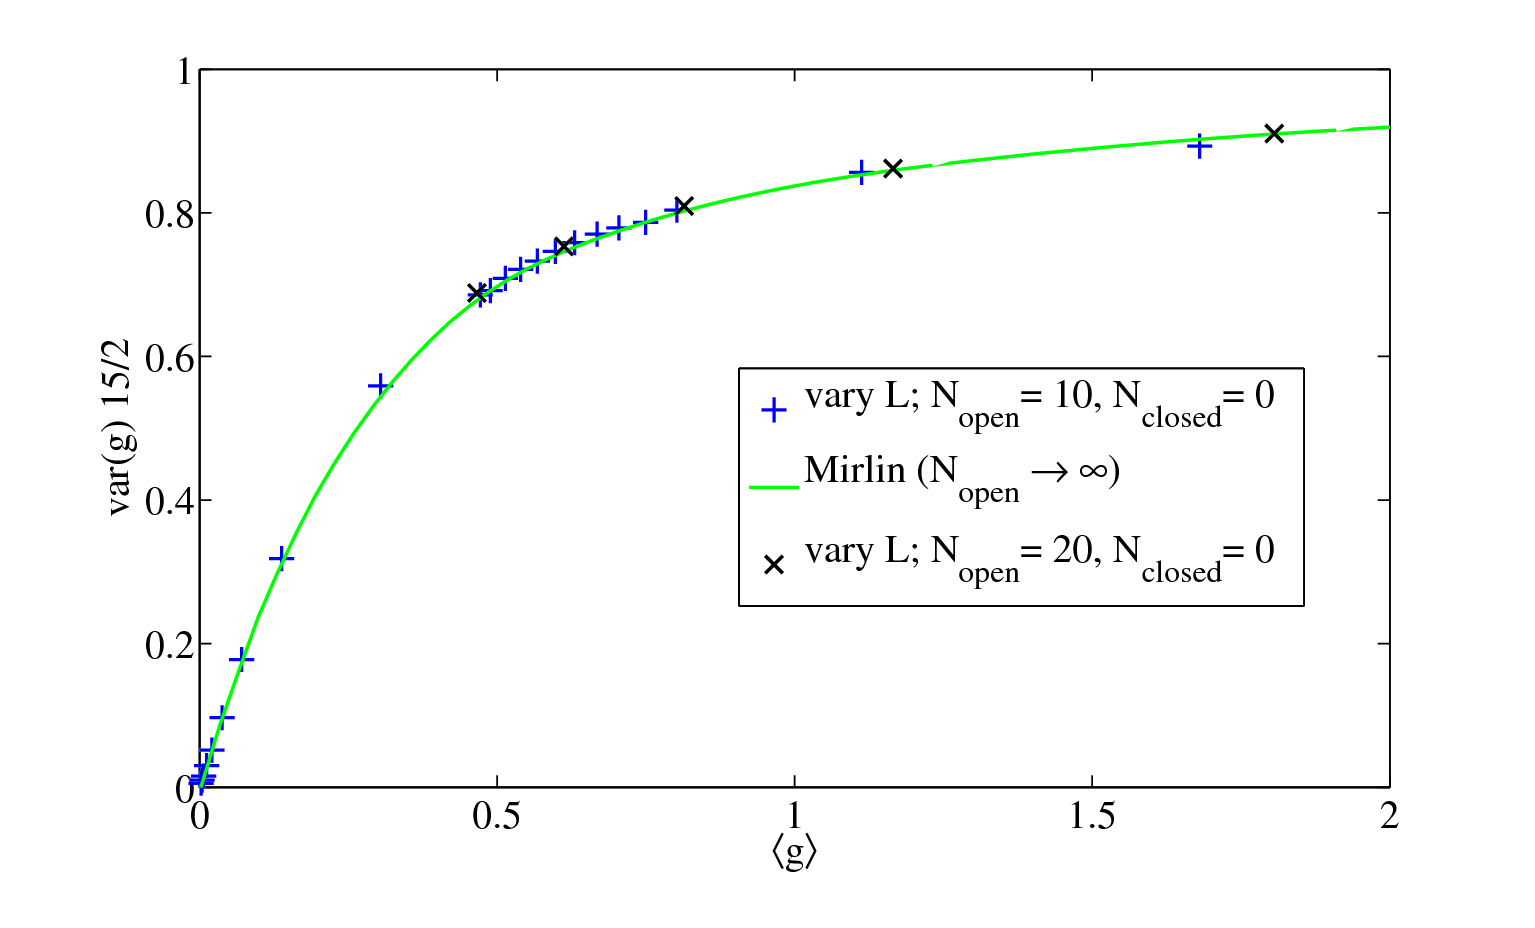
\includegraphics{pictures/var_g_versus_g_no_closed_channels}}
}
\vskip -0.5cm
% NOTE:Lorem ipsum dolor sit amet, consectetur adipiscing elit; Maecenas ultrices egestas commodo, use
%\caption[short desk]{long desk}
\caption[Position-dependent diffusion coefficient~$D(z)$ as predicted by self- consistent theory of localization (smooth red curves) and numeric results (rough blue lines) for quasi-1D waveguides with randomly-Lorem ipsum dolor sit amet, consectetur adipiscing elit; Maecenas ultrices egestas commodo~$L$, constant scatterer density, and width~$W$.]{Position-dependent diffusion coefficient $D(z)$ as predicted by self-consistent theory of localization (smooth red curves) and numeric results (rough blue lines) for quasi-1D waveguides with randomly-Lorem ipsum dolor sit amet, consectetur adipiscing elit; Maecenas ultrices egestas commodo~$L$, constant scatterer density, and width~$W$. Very good agreement for ballistic ($L=100 \lambda$), diffusive, and localized ($L=800 \lambda$) regimes. The term $\ell$ is transport mean free path, and $z_0$ is penetration depth.}
\label{fig:Dz_passive}
\end{figure}

%Method:Lorem ipsum dolor sit amet, consectetur adipiscing elit; Maecenas ultrices egestas commodo?}
Lorem ipsum dolor sit amet, consectetur adipiscing elit; Maecenas ultrices egestas commodo,Lorem ipsum dolor sit amet, consectetur adipiscing elit; Maecenas ultrices egestas commodo~\cite{1981_MacKinnon_scaling,1992_Pendry,2003_Kettemann} 
% note: when MacKinnon cites tmm, he uses 1981_MacKinnon_scaling and 
% MacKinnon A 1994 J. Phys. Condensed Matter 6, 2511
for the entire waveguide. Essentially,Lorem ipsum dolor sit amet, consectetur adipiscing elit; Maecenas ultrices egestas commodo. Not only is the quasi-1D geometry experimentally viable~\cite{2009_Genack_PRB},Lorem ipsum dolor sit amet, consectetur adipiscing elit; Maecenas ultrices egestas commodo~\cite{1982_Dorokhov_DMPK,1988_Mello_Kumar_DMPK}. Here, waveguides described as ``quasi-1D'' have the following characteristics: (1)~Lorem ipsum dolor sit amet, consectetur adipiscing elit; Maecenas ultrices egestas commodo, expressed as $E(y=0,W;\forall z)=0$ as for metallic edges, (2)~waveguide width $W$ less than $\ell_{tmfp}$Lorem ipsum dolor sit amet, consectetur adipiscing elit; Maecenas ultrices egestas commodo, and (3)~aspect ratio ($L:W$) is not fixed (i.e., $W$ is constant when $L$ is increased, with a fixed disorder density). Further,Lorem ipsum dolor sit amet, consectetur adipiscing elit; Maecenas ultrices egestas commodo.

As shown in Appendix~\ref{sec:appendix_derivation_transfer_matrices_quasi1d}, the differential wave equation
\begin{equation}
\nabla^2 E(\vec{r}) = - \frac{\omega^2}{c^2} E(\vec{r})
\label{eq:wave_equation_electric_field_introduction}
\end{equation}
Lorem ipsum dolor sit amet, consectetur adipiscing elit; Maecenas ultrices egestas commodo(resolving wave vector $\vec{k}$ into $k_{\perp}$ and $k_{\parallel}$).Lorem ipsum dolor sit amet, consectetur adipiscing elit; Maecenas ultrices egestas commodo, scattering potentials are introduced, initially as $\delta$ functions.Lorem ipsum dolor sit amet, consectetur adipiscing elit; Maecenas ultrices egestas commodo\textit{ab initio} based on Maxwell's equations~\cite{1999_Jackson},Lorem ipsum dolor sit amet, consectetur adipiscing elit; Maecenas ultrices egestas commodo. 

For light waves,Lorem ipsum dolor sit amet, consectetur adipiscing elit; Maecenas ultrices egestas commodo
form of a vector.Lorem ipsum dolor sit amet, consectetur adipiscing elit; Maecenas ultrices egestas commodo-Lorem ipsum dolor sit amet, consectetur adipiscing elit; Maecenas ultrices egestas commodo,Lorem ipsum dolor sit amet, consectetur adipiscing elit; Maecenas ultrices egestas commodo(c.f. Appendix~\ref{sec:appendix_derivation_transfer_matrices_quasi1d}). In 1D,Lorem ipsum dolor sit amet, consectetur adipiscing elit; Maecenas ultrices egestas commodo$E_0$ and its derivative $E_0^{\prime}$Lorem ipsum dolor sit amet, consectetur adipiscing elit; Maecenas ultrices egestas commodo$\Delta x$:
\begin{equation}
 \left( \begin{array}{cc}
t_{11} & t_{12} \\
t_{21} & t_{22} \\
\end{array} \right)
\left( \begin{array}{c}
E_0 \\
E_0^{\prime}
\end{array} \right)
=
\left( \begin{array}{c}
E_{\Delta x} \\
E_{\Delta x}^{\prime}
\end{array} \right).
\end{equation}
Lorem ipsum dolor sit amet, consectetur adipiscing elit; Maecenas ultrices egestas commodo$\hat{T}_{total} = \prod_i \hat{T}_i$.Lorem ipsum dolor sit amet, consectetur adipiscing elit; Maecenas ultrices egestas commodo.Lorem ipsum dolor sit amet, consectetur adipiscing elit; Maecenas ultrices egestas commodo,Lorem ipsum dolor sit amet, consectetur adipiscing elit; Maecenas ultrices egestas commodo$\delta$ function.Lorem ipsum dolor sit amet, consectetur adipiscing elit; Maecenas ultrices egestas commodo, the resulting electric field magnitude, plotted in Fig.~\ref{fig:electric_field_zoomed}, is a secondary benefit.

\begin{figure}
\vskip -0.5cm
\centerline{
\scalebox{.5}{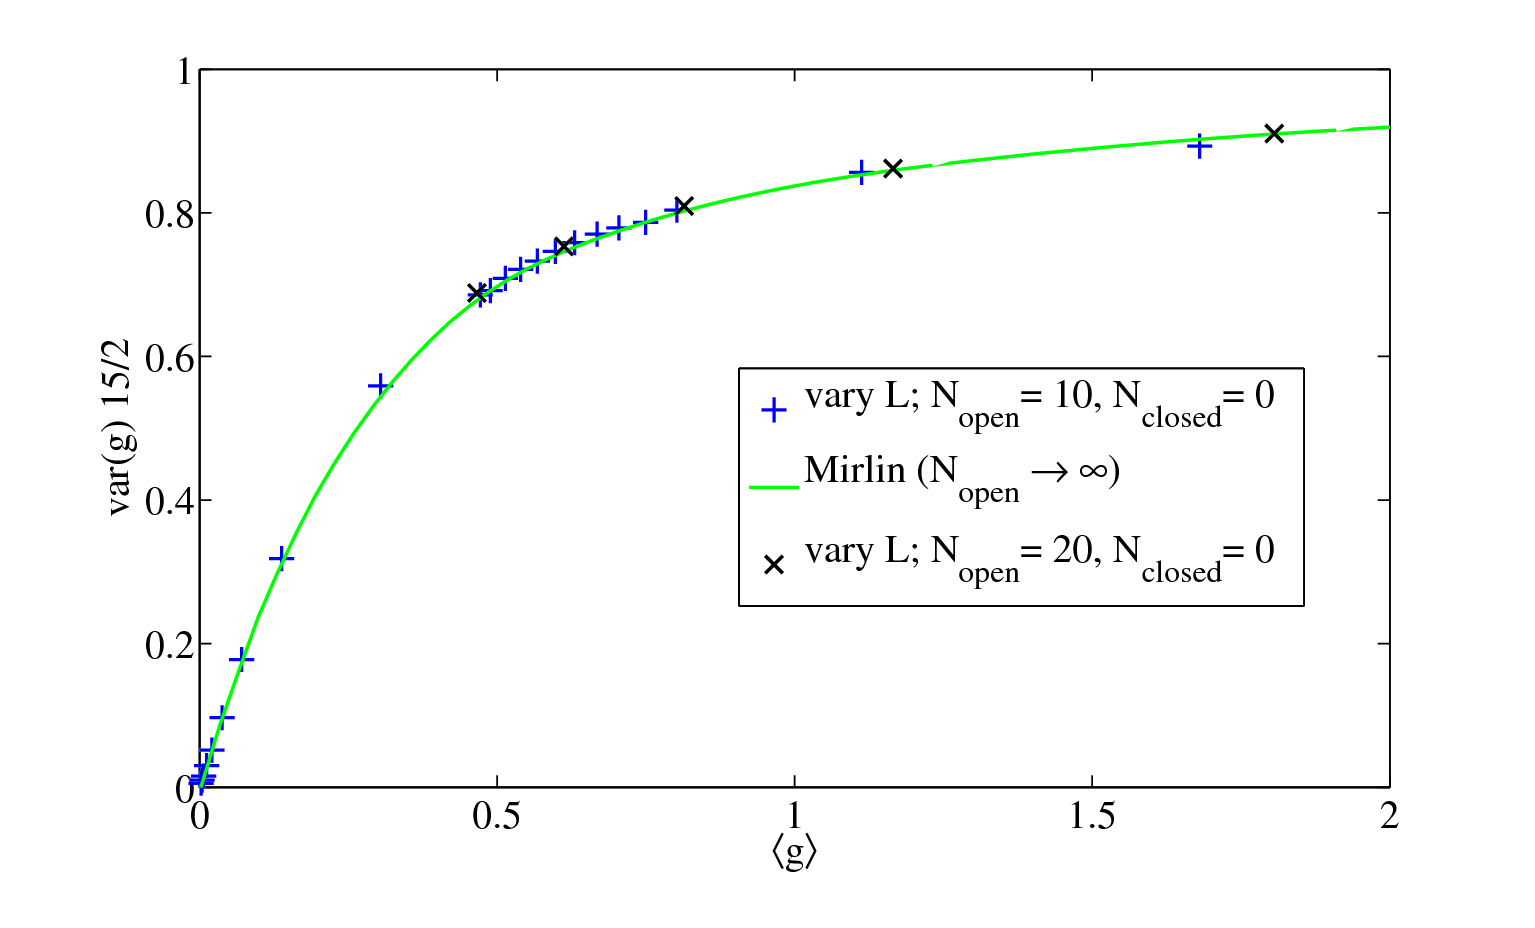
\includegraphics{pictures/var_g_versus_g_no_closed_channels}}
}
\vskip -0.5cm
% NOTE:Lorem ipsum dolor sit amet, consectetur adipiscing elit; Maecenas ultrices egestas commodo, use
%\caption[short desk]{long desk}
\caption[Lorem ipsum dolor sit amet, consectetur adipiscing elit; Maecenas ultrices egestas commodo-1Lorem ipsum dolor sit amet, consectetur adipiscing elit; Maecenas ultrices egestas commodo.]{Lorem ipsum dolor sit amet, consectetur adipiscing elit; Maecenas ultrices egestas commodo-1Lorem ipsum dolor sit amet, consectetur adipiscing elit; Maecenas ultrices egestas commodo. Midsection of waveguide is shown (from $z/L=80/200$ to $z=120/200$) for a resonant frequency (higher than average transmission). Spatially varying field intensity (with continuous wave incident flux)Lorem ipsum dolor sit amet, consectetur adipiscing elit; Maecenas ultrices egestas commodo,Lorem ipsum dolor sit amet, consectetur adipiscing elit; Maecenas ultrices egestas commodo.
\label{fig:electric_field_zoomed}}
% The Poynting vector can plotted
% [don't say this because you aren'Lorem ipsum dolor sit amet, consectetur adipiscing elit; Maecenas ultrices egestas commodo.]
\end{figure}

Lorem ipsum dolor sit amet, consectetur adipiscing elit; Maecenas ultrices egestas commodo~\cite{2007_Froufe-Perez_PRE},Lorem ipsum dolor sit amet, consectetur adipiscing elit; Maecenas ultrices egestas commodo.Lorem ipsum dolor sit amet, consectetur adipiscing elit; Maecenas ultrices egestas commodo~\cite{1968_Osedelec}.
% A simple showing of this would be nice
Lorem ipsum dolor sit amet, consectetur adipiscing elit; Maecenas ultrices egestas commodo. % (due to conservation of flux?) 
Lorem ipsum dolor sit amet, consectetur adipiscing elit; Maecenas ultrices egestas commodo
%citation would be nice here,Lorem ipsum dolor sit amet, consectetur adipiscing elit; Maecenas ultrices egestas commodo
%\begin{equation}
$\rm{det}(\hat{A})\rm{det}(\hat{B})=\rm{det}(\hat{A}\hat{B})$.
%\end{equation}
A self-Lorem ipsum dolor sit amet, consectetur adipiscing elit; Maecenas ultrices egestas commodo~\cite{1999_yamilov_selfembed,1976_Bellman_Wing_embedding}.
%Although self-Lorem ipsum dolor sit amet, consectetur adipiscing elit; Maecenas ultrices egestas commodo, it is applied here to waveguides. %1D and planar quasi-1D waveguide geometries.
%In passive media, conservation of energy implies $T+R=1$Lorem ipsum dolor sit amet, consectetur adipiscing elit; Maecenas ultrices egestas commodo.
Lorem ipsum dolor sit amet, consectetur adipiscing elit; Maecenas ultrices egestas commodo-Lorem ipsum dolor sit amet, consectetur adipiscing elit; Maecenas ultrices egestas commodo$\langle g \rangle$ versus variance var$(g)$Lorem ipsum dolor sit amet, consectetur adipiscing elit; Maecenas ultrices egestas commodo-based approach~\cite{2000_Mirlin}. With no fitting parameters, there is very good agreement (c.f. Fig.~\ref{fig:Mirlin_supersymmetry_g_varg}). Similarly,Lorem ipsum dolor sit amet, consectetur adipiscing elit; Maecenas ultrices egestas commodo$D(z)$ (c.f. Fig.~\ref{fig:Dz_passive}).

\begin{figure}
\vskip -0.5cm
\centerline{
\scalebox{.45}{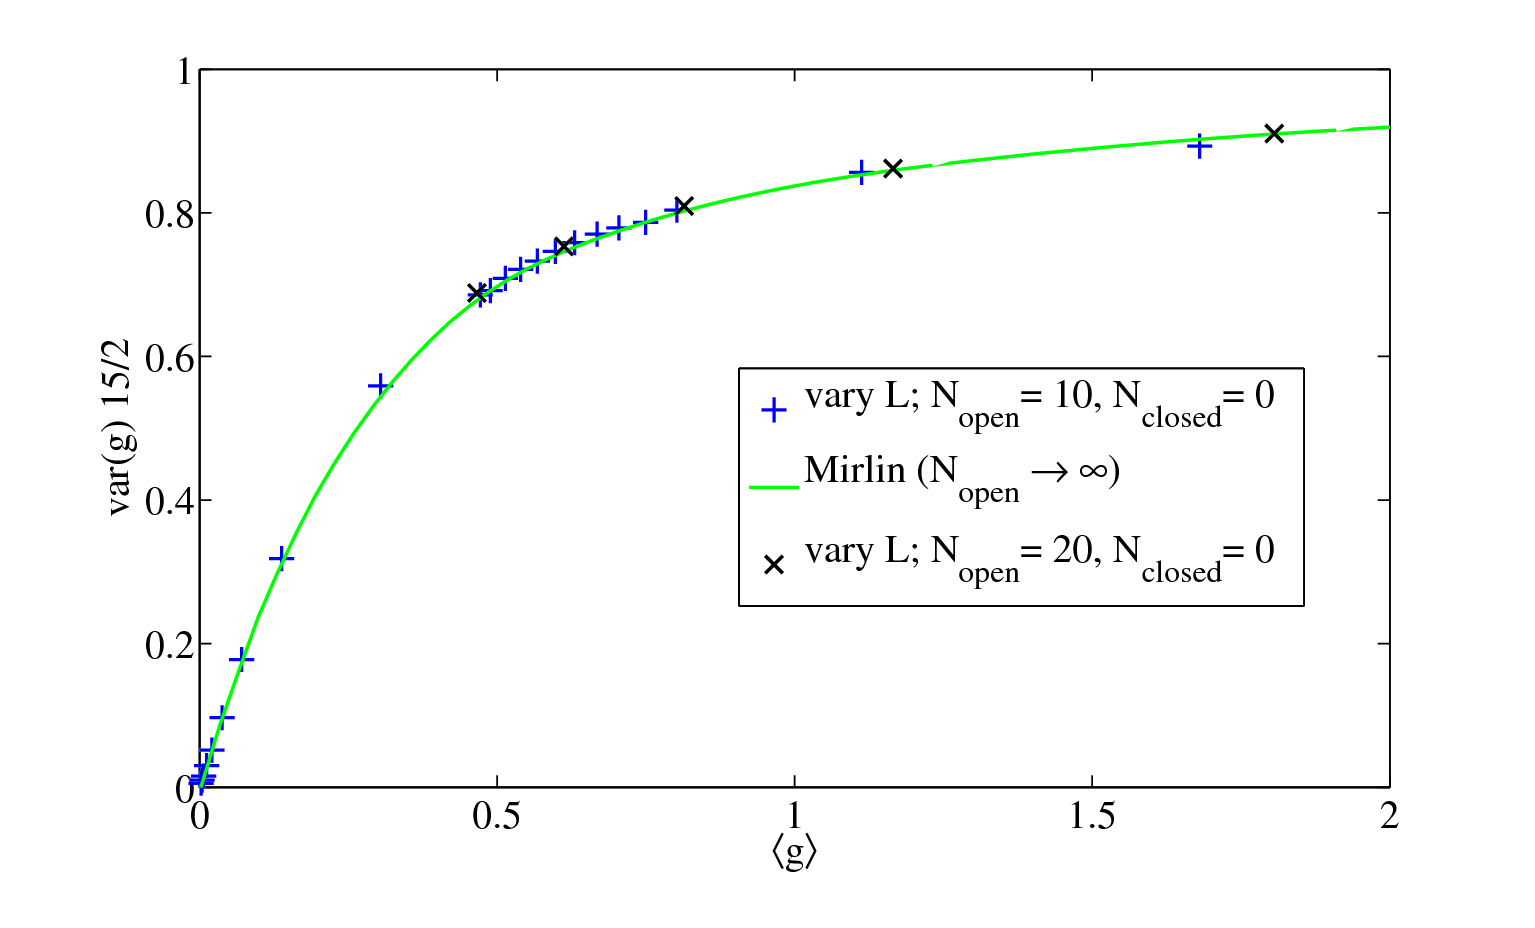
\includegraphics{pictures/var_g_versus_g_no_closed_channels}}
}
\vskip -0.5cm
% NOTE:Lorem ipsum dolor sit amet, consectetur adipiscing elit; Maecenas ultrices egestas commodo, use
%\caption[short desk]{long desk}
\caption[Lorem ipsum dolor sit amet, consectetur adipiscing elit; Maecenas ultrices egestas commodo$g$ versus variance of $g$ for quasi-1D waveguide~\cite{2000_Mirlin}Lorem ipsum dolor sit amet, consectetur adipiscing elit; Maecenas ultrices egestas commodo~\ref{sec:method_numerical}.]{Lorem ipsum dolor sit amet, consectetur adipiscing elit; Maecenas ultrices egestas commodo$g$ versus variance of $g$ for quasi-1D waveguide~\cite{2000_Mirlin}Lorem ipsum dolor sit amet, consectetur adipiscing elit; Maecenas ultrices egestas commodo~\ref{sec:method_numerical}.Lorem ipsum dolor sit amet, consectetur adipiscing elit; Maecenas ultrices egestas commodo. The $15/2$Lorem ipsum dolor sit amet, consectetur adipiscing elit; Maecenas ultrices egestas commodo.Lorem ipsum dolor sit amet, consectetur adipiscing elit; Maecenas ultrices egestas commodo$\langle g \rangle$ and var$(g)$Lorem ipsum dolor sit amet, consectetur adipiscing elit; Maecenas ultrices egestas commodo(with the number of open channels $N_{open}$ determined by $W$) and varying system length $L$. The supersymmetry-Lorem ipsum dolor sit amet, consectetur adipiscing elit; Maecenas ultrices egestas commodo, but $N_{open}$ equal to 10 and 20 is sufficient.\label{fig:Mirlin_supersymmetry_g_varg}}
\end{figure}
  

\section{OUTLINE OF TRANSPORT REGIMES}
\label{sec:twod_plot}

Lorem ipsum dolor sit amet, consectetur adipiscing elit; Maecenas ultrices egestas commodo, a two-parameter diagram (c.f.~Fig.~\ref{fig:regime_plot_main})  % Spring semester 2009, Ben and Dr Yamilov
enumerates types of transport behavior. The first parameter is system length $L$,Lorem ipsum dolor sit amet, consectetur adipiscing elit; Maecenas ultrices egestas commodo.Lorem ipsum dolor sit amet, consectetur adipiscing elit; Maecenas ultrices egestas commodo. The two-Lorem ipsum dolor sit amet, consectetur adipiscing elit; Maecenas ultrices egestas commodo.Lorem ipsum dolor sit amet, consectetur adipiscing elit; Maecenas ultrices egestas commodo$T/{\cal E}$ in nonconservative random media.

A single-valued parameter such as~$T/{\cal E}$ is useful even in this two-Lorem ipsum dolor sit amet, consectetur adipiscing elit; Maecenas ultrices egestas commodo. However, not all single-Lorem ipsum dolor sit amet, consectetur adipiscing elit; Maecenas ultrices egestas commodo.Lorem ipsum dolor sit amet, consectetur adipiscing elit; Maecenas ultrices egestas commodo~$T/{\cal E}$,Lorem ipsum dolor sit amet, consectetur adipiscing elit; Maecenas ultrices egestas commodo. Currently,Lorem ipsum dolor sit amet, consectetur adipiscing elit; Maecenas ultrices egestas commodo.

%\section{what is the plan?}
Figure~\ref{fig:regime_plot_main} describes types of transport in quasi-1D waveguides with random media; it has three passive regimes: ballistic (\textbf{B}), diffusive (\textbf{D}), localized (\textbf{L}) on the horizontal axis and gain (\textbf{G}) or absorption (\textbf{A}) strength on the vertical axis. The two-Lorem ipsum dolor sit amet, consectetur adipiscing elit; Maecenas ultrices egestas commodo. The passive regime transitions (B/D/L)Lorem ipsum dolor sit amet, consectetur adipiscing elit; Maecenas ultrices egestas commodo~$\ell_{tmfp}$ and localization length~$\xi$, as described in section \ref{sec:thesis_statement}.Lorem ipsum dolor sit amet, consectetur adipiscing elit; Maecenas ultrices egestas commodo~$\lambda$. 

\begin{figure}[t]
\vskip -.8cm 
\centerline{
\scalebox{.65}{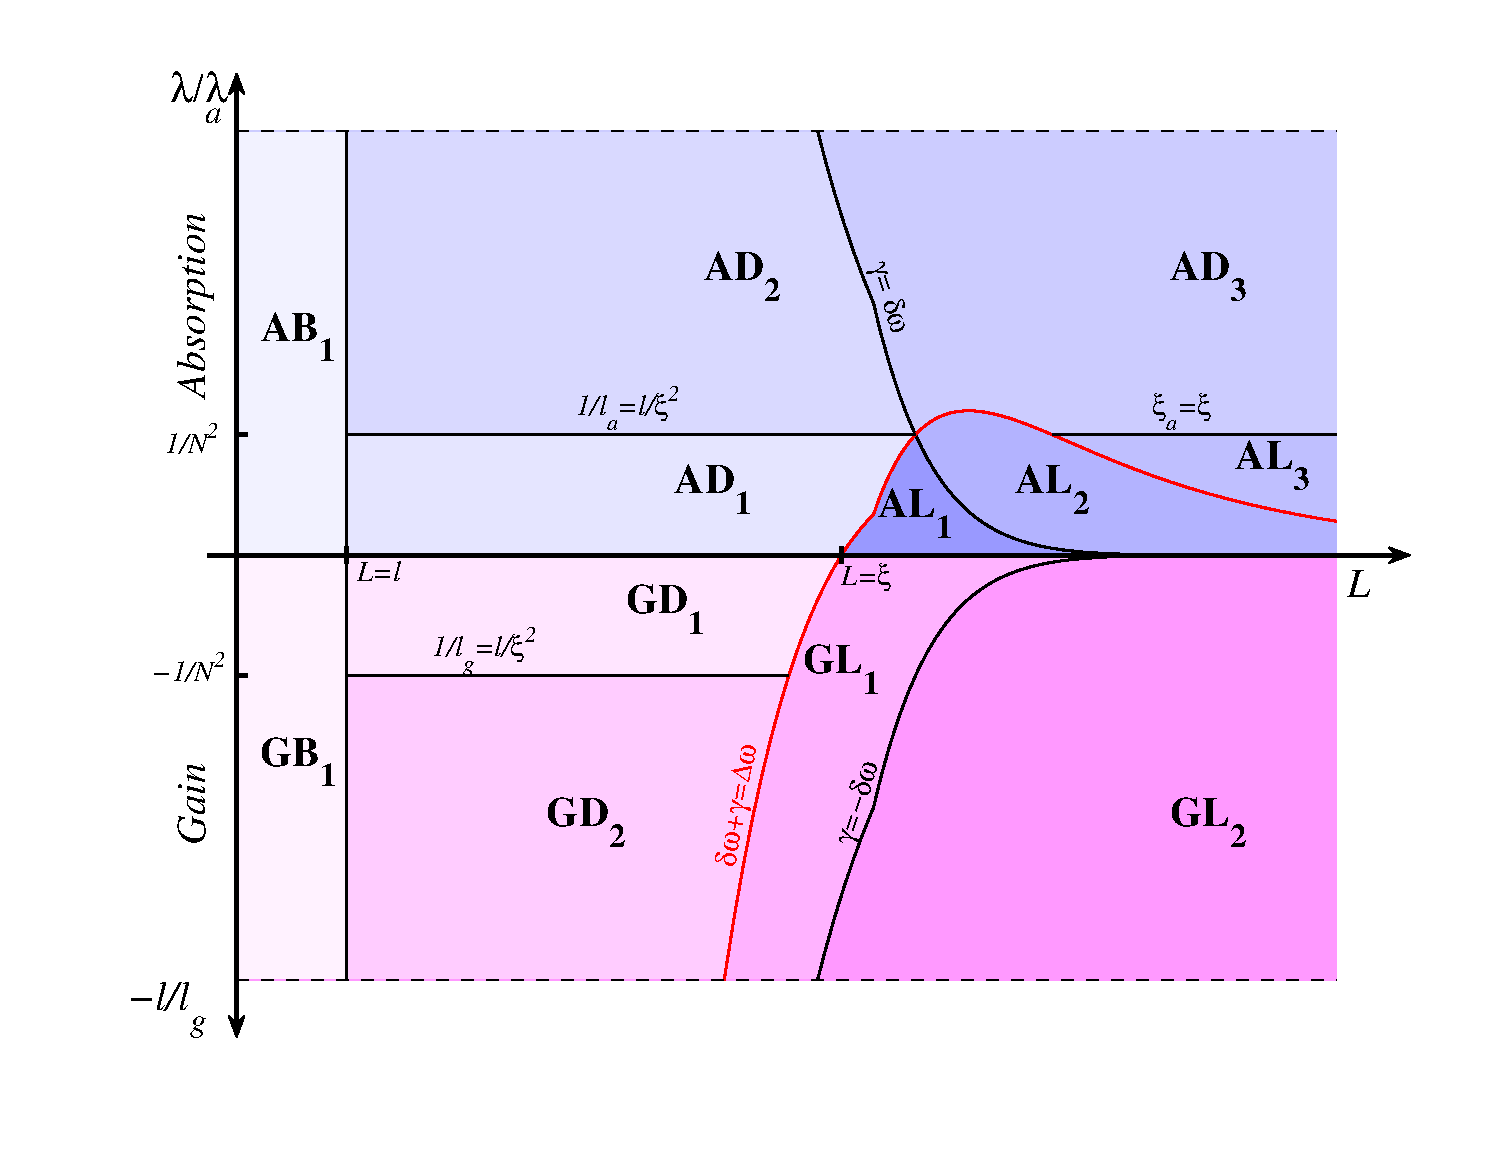
\includegraphics{pictures/regimes_plot_main}}
}
\vskip -0.5cm
\caption[Lorem ipsum dolor sit amet, consectetur adipiscing elit; Maecenas ultrices egestas commodo-letter abbreviations (see text for explanation).]{Lorem ipsum dolor sit amet, consectetur adipiscing elit; Maecenas ultrices egestas commodo-letter abbreviations (see text for explanation).Lorem ipsum dolor sit amet, consectetur adipiscing elit; Maecenas ultrices egestas commodo. Passive (conservative)Lorem ipsum dolor sit amet, consectetur adipiscing elit; Maecenas ultrices egestas commodo,Lorem ipsum dolor sit amet, consectetur adipiscing elit; Maecenas ultrices egestas commodo$L$. Plotted vertically, amounts of absorption or gain (nonconservative media)Lorem ipsum dolor sit amet, consectetur adipiscing elit; Maecenas ultrices egestas commodo. 
%Regime plot for quasi-1D random media.Lorem ipsum dolor sit amet, consectetur adipiscing elit; Maecenas ultrices egestas commodo; each region is denoted by a two-letter abbreviation. See text for explanation.
\label{fig:regime_plot_main}
}
\end{figure}

%Lorem ipsum dolor sit amet, consectetur adipiscing elit; Maecenas ultrices egestas commodo. For example, 
%For brevity, only absorption is referred to,Lorem ipsum dolor sit amet, consectetur adipiscing elit; Maecenas ultrices egestas commodo. 
The absorption (gain) rate $\gamma_{a,g}$Lorem ipsum dolor sit amet, consectetur adipiscing elit; Maecenas ultrices egestas commodo,Lorem ipsum dolor sit amet, consectetur adipiscing elit; Maecenas ultrices egestas commodo(doubled) along a specific path. The absorption (gain) rate is the inverse of the absorption (gain) lifetime, 
%\begin{equation}
$\gamma_{a,g} = \frac{1}{\tau_{a,g}}$, 
%\end{equation}
where $\tau_{a,g}$Lorem ipsum dolor sit amet, consectetur adipiscing elit; Maecenas ultrices egestas commodo(doubled).Lorem ipsum dolor sit amet, consectetur adipiscing elit; Maecenas ultrices egestas commodo. Given a characteristic time $\tau_{a,g}$,Lorem ipsum dolor sit amet, consectetur adipiscing elit; Maecenas ultrices egestas commodo
%\begin{equation}
$\ell_{a,g} = \tau_{a,g} c$, 
%\end{equation}
where $c$Lorem ipsum dolor sit amet, consectetur adipiscing elit; Maecenas ultrices egestas commodo.Lorem ipsum dolor sit amet, consectetur adipiscing elit; Maecenas ultrices egestas commodo(doubling) with respect to the path length. The $\ell_{a,g}$ is determined from the time-Lorem ipsum dolor sit amet, consectetur adipiscing elit; Maecenas ultrices egestas commodo,
\begin{equation}
D \frac{\partial^2 I}{\partial z^2} = \frac{\partial I}{\partial t},
\label{eq:diffusion_equation_1D}
\end{equation}
to be 
% see /svn/bens/lab_notebook/20090422_dr_Yamilov_mtg_regime_change_for_plot.pdf
% equation 37
\begin{equation}
\ell_{a,g}= \left( \frac{d}{\pi^2}\right) \frac{L^2}{\ell_{tmfp}}.
\label{eq:ballistic_gain_abs}
\end{equation}
However, $\ell_{a,g}$Lorem ipsum dolor sit amet, consectetur adipiscing elit; Maecenas ultrices egestas commodo(doubled when gain is present). The system length $L$ (Lorem ipsum dolor sit amet, consectetur adipiscing elit; Maecenas ultrices egestas commodo) should be replaced by a new diffusive-regime length, $\xi_{a,g}$. Eq.~\ref{eq:ballistic_gain_abs} can then be solved for $\xi_{a,g}$:
\begin{equation}
 \xi_{a,g} = \sqrt{\frac{\ell_{a,g} \ell_{tmfp}}{d}}.
\label{eq:diffusive_absorption_length}
\end{equation}
Physically, $\xi_{a,g}$Lorem ipsum dolor sit amet, consectetur adipiscing elit; Maecenas ultrices egestas commodo-scattering system. To distinguish the two absorption (gain) lengths, $\xi_{a,g}$Lorem ipsum dolor sit amet, consectetur adipiscing elit; Maecenas ultrices egestas commodo$L$ (rather than path length $L_D$), whereas $\ell_{a,g}$Lorem ipsum dolor sit amet, consectetur adipiscing elit; Maecenas ultrices egestas commodo$L_D$. If $L$ is equal to $L_D$, then no diffusion is occurring and $\ell_{a,g}$ is equal to $\xi_{a,g}$. Usually,Lorem ipsum dolor sit amet, consectetur adipiscing elit; Maecenas ultrices egestas commodo$L_D$Lorem ipsum dolor sit amet, consectetur adipiscing elit; Maecenas ultrices egestas commodo$L$.Lorem ipsum dolor sit amet, consectetur adipiscing elit; Maecenas ultrices egestas commodo: first, experimentally, $L_D$ is harder to measure than $L$; second,Lorem ipsum dolor sit amet, consectetur adipiscing elit; Maecenas ultrices egestas commodo.

For localized systems,Lorem ipsum dolor sit amet, consectetur adipiscing elit; Maecenas ultrices egestas commodo(i.e., ray optics do not apply). In this regime $\xi_{a,g}$ is used, but it is not defined in terms of $\ell_{a,g}$ as in Eq.~\ref{eq:diffusive_absorption_length}.Lorem ipsum dolor sit amet, consectetur adipiscing elit; Maecenas ultrices egestas commodo$\xi_{a} = \xi$ (the horizontal line between $AD_3$ and $AL_3$ in Fig.~\ref{fig:regime_plot_main}).Lorem ipsum dolor sit amet, consectetur adipiscing elit; Maecenas ultrices egestas commodo.~\ref{eq:diffusive_absorption_length} to $\xi_{a,g} = \xi = N_{open} \ell_{tmfp}$ and solving 
\begin{equation}
N_{open}^2 \ell_{tmfp}^2 = \frac{\ell_{tmfp}\ell_{a,g}}{d}
\end{equation}
to get $\ell_{a,g} =d N_{open}^2 \ell_{tmfp}$. For the diffusive regime,Lorem ipsum dolor sit amet, consectetur adipiscing elit; Maecenas ultrices egestas commodo(gain)Lorem ipsum dolor sit amet, consectetur adipiscing elit; Maecenas ultrices egestas commodo. The remaining curves in Fig.~\ref{fig:regime_plot_main}Lorem ipsum dolor sit amet, consectetur adipiscing elit; Maecenas ultrices egestas commodo, rather than the characteristic lengths.

For passive media,Lorem ipsum dolor sit amet, consectetur adipiscing elit; Maecenas ultrices egestas commodo($\delta \omega$ of the Thouless criterion in Eq.~\ref{eq:Thouless_passive})Lorem ipsum dolor sit amet, consectetur adipiscing elit; Maecenas ultrices egestas commodo(Lorem ipsum dolor sit amet, consectetur adipiscing elit; Maecenas ultrices egestas commodo). To account for absorption or gain, an additional term is needed~\cite{2005_Yamilov_correlations} in the form of a rate: 
%\begin{equation}
$\delta \omega +\gamma_{a,g}$.
%\end{equation}
Although the width of DOS $\Delta \omega$Lorem ipsum dolor sit amet, consectetur adipiscing elit; Maecenas ultrices egestas commodo-Kronig relation~\cite{1999_Jackson},Lorem ipsum dolor sit amet, consectetur adipiscing elit; Maecenas ultrices egestas commodo. 
% boundaries
Lorem ipsum dolor sit amet, consectetur adipiscing elit; Maecenas ultrices egestas commodo(Lorem ipsum dolor sit amet, consectetur adipiscing elit; Maecenas ultrices egestas commodo\cite{1968_Letokhov}) or absorption rate $\gamma_{a,g}=\mp~c/\ell_{a,g}$:
\begin{equation}
\delta'=\frac{\delta \omega +\gamma_{a,g}}{\Delta \omega};
\label{eq:generalized_thouless}
\end{equation}
it is plotted as the red curve $\delta'=1$. Physically,Lorem ipsum dolor sit amet, consectetur adipiscing elit; Maecenas ultrices egestas commodo-Lorem ipsum dolor sit amet, consectetur adipiscing elit; Maecenas ultrices egestas commodo.Lorem ipsum dolor sit amet, consectetur adipiscing elit; Maecenas ultrices egestas commodo-mode of the system, as plotted by the black curve $\pm \gamma = \delta \omega$. %Lorem ipsum dolor sit amet, consectetur adipiscing elit; Maecenas ultrices egestas commodo. For example, in the diffusive regime, $L$, $\xi$, $\ell_{tmfp}$, and $\ell_{a,g}$Lorem ipsum dolor sit amet, consectetur adipiscing elit; Maecenas ultrices egestas commodo. 
%Lorem ipsum dolor sit amet, consectetur adipiscing elit; Maecenas ultrices egestas commodo,Lorem ipsum dolor sit amet, consectetur adipiscing elit; Maecenas ultrices egestas commodo.
% caveat
Lorem ipsum dolor sit amet, consectetur adipiscing elit; Maecenas ultrices egestas commodo.~\ref{fig:regime_plot_main},Lorem ipsum dolor sit amet, consectetur adipiscing elit; Maecenas ultrices egestas commodo.Lorem ipsum dolor sit amet, consectetur adipiscing elit; Maecenas ultrices egestas commodo, two-Lorem ipsum dolor sit amet, consectetur adipiscing elit; Maecenas ultrices egestas commodo.

% transport behavior of each regime
In the ballistic regime $GB_1$,Lorem ipsum dolor sit amet, consectetur adipiscing elit; Maecenas ultrices egestas commodo(and similarly for $AB_1$ when $\ell_a < L$).Lorem ipsum dolor sit amet, consectetur adipiscing elit; Maecenas ultrices egestas commodo$AD_1$ and $GD_1$,Lorem ipsum dolor sit amet, consectetur adipiscing elit; Maecenas ultrices egestas commodo. The use of conditional statistics~\cite{2005_Yamilov_correlations}Lorem ipsum dolor sit amet, consectetur adipiscing elit; Maecenas ultrices egestas commodo. With sufficient absorption, signatures of diffusion are reduced ($AD_2$) and suppressed ($AD_3$). In contrast, gain enhances fluctuations ($GL_1$) and leads to lasing ($GL_2$) on average for many realizations~\cite{1968_Letokhov}. Transport in region $GD_2$ is the equivalent of ``negative absorption'' in region $AD_2$.Lorem ipsum dolor sit amet, consectetur adipiscing elit; Maecenas ultrices egestas commodo($AL_1$)Lorem ipsum dolor sit amet, consectetur adipiscing elit; Maecenas ultrices egestas commodo($AL_2$)Lorem ipsum dolor sit amet, consectetur adipiscing elit; Maecenas ultrices egestas commodo($AL_3$).

% the hump of AL_2 is not separated because?

%Lorem ipsum dolor sit amet, consectetur adipiscing elit; Maecenas ultrices egestas commodo's projections\cite{2000_Mirlin} in the localized regime.


% if I only have 10 minutes of the presentation, I will not have time for these regions
\begin{comment}
\begin{figure}
\vskip -0.5cm
\centerline{
\scalebox{.75}{\includegraphics{pictures/regimes_plot_upper}}}
\vskip -0.5cm
%\caption[Upper regime plot (strong absorption) for quasi-1D random media.]{Upper regime plot (strong absorption) for quasi-1D random media.Lorem ipsum dolor sit amet, consectetur adipiscing elit; Maecenas ultrices egestas commodo. See text for explanation.}
\label{fig:regime_plot_upper}
\end{figure}

\begin{figure}
\vskip -0.5cm
\centerline{
\scalebox{.75}{\includegraphics{pictures/regimes_plot_lower}}}
\vskip -0.5cm
%\caption{[Lower regime plot (strong gain) for quasi-1D random media.]Lower regime plot (strong gain) for quasi-1D random media. See text for explanation.}
\label{fig:regime_plot_lower}
\end{figure}
\end{comment}

% Note: analytical quasi-1D solution found by~\cite{1994_Beenakker_exact}

%Lorem ipsum dolor sit amet, consectetur adipiscing elit; Maecenas ultrices egestas commodo(numerical model) and the plan is detailed and well-defined. Also, it is not too broad or too narrow.

Lorem ipsum dolor sit amet, consectetur adipiscing elit; Maecenas ultrices egestas commodo.~\ref{fig:regime_plot_main},Lorem ipsum dolor sit amet, consectetur adipiscing elit; Maecenas ultrices egestas commodo$T/{\cal E}$.Lorem ipsum dolor sit amet, consectetur adipiscing elit; Maecenas ultrices egestas commodo$D(z)$, correlation functions, and the inverse participation ratio,Lorem ipsum dolor sit amet, consectetur adipiscing elit; Maecenas ultrices egestas commodo.Lorem ipsum dolor sit amet, consectetur adipiscing elit; Maecenas ultrices egestas commodo~\cite{2010_Payne_closed}, wave front shaping~\cite{2008_Vellekoop_Mosk}Lorem ipsum dolor sit amet, consectetur adipiscing elit; Maecenas ultrices egestas commodo, eigenmodes of transmission~\cite{1986_Imry},Lorem ipsum dolor sit amet, consectetur adipiscing elit; Maecenas ultrices egestas commodo.Lorem ipsum dolor sit amet, consectetur adipiscing elit; Maecenas ultrices egestas commodo.
